\documentclass[11pt,a4paper]{article}

\usepackage[utf8]{inputenc}
\usepackage[T1]{fontenc}
\usepackage[french]{babel}
\usepackage{xcolor}
\usepackage{graphicx}
\usepackage{float}
\usepackage{booktabs}
\usepackage{hyperref}
\usepackage{geometry}
\usepackage{titlesec}
\usepackage{fancyhdr}

\geometry{margin=2.5cm}
\hypersetup{colorlinks=true, linkcolor=blue!50!black, urlcolor=blue!50!black}

\pagestyle{fancy}
\fancyhf{}
\fancyhead[L]{Génération JSON et mot-clé \texttt{not}}
\fancyhead[R]{\thepage}
\renewcommand{\headrulewidth}{0.4pt}

\title{Génération de données JSON par un LLM : le cas du mot-clé \texttt{not}}
\author{Zein Mil \\ Licence 3 IM2D, Université Paris-Dauphine}
\date{\today}

\begin{document}

\begin{titlepage}
\centering
\vspace*{1cm}

{\large\scshape Université Paris-Dauphine (PSL)\par}
\vspace{0.15cm}
{\normalsize Licence 3 --- Informatique, Mathématiques et Décision (IM2D)\par}

\vspace{0.4cm}
\rule{0.6\textwidth}{0.4pt}
\vspace{2.5cm}

{\Large\itshape Rapport de stage\par}
\vspace{1cm}

\rule{\textwidth}{1pt}
\vspace{0.5cm}
{\huge\bfseries Génération de données JSON\\[0.3cm] par un LLM\par}
\vspace{0.5cm}
{\Large le cas du mot-clé \texttt{not}\par}
\vspace{0.5cm}
\rule{\textwidth}{1pt}

\vspace{3cm}

\begin{minipage}{0.45\textwidth}
\begin{flushleft} \large
\textbf{Étudiante}\\
Zein Mil
\end{flushleft}
\end{minipage}
\begin{minipage}{0.45\textwidth}
\begin{flushright} \large
\textbf{Maître de stage}\\
Dario Colazzo\\[0.5cm]
\textbf{Encadrante}\\
Nour Ben Ali
\end{flushright}
\end{minipage}

\vspace{2cm}
\rule{0.3\textwidth}{0.4pt}

\vfill

{\large \today\par}

\end{titlepage}

\tableofcontents
\newpage

\section*{Présentation}
\addcontentsline{toc}{section}{Présentation}

Étudiante en licence 3 IM2D à l'Université Paris-Dauphine, j'ai réalisé ce travail dans le cadre de mon stage, sous la direction de mon maître de stage Dario Colazzo et avec l'encadrement de Nour Ben Ali. Ce rapport présente l'ensemble des travaux menés depuis le début du stage, depuis les premières expérimentations jusqu'aux résultats les plus récents.

\section{Le sujet du stage}

Ce travail porte sur les modèles de langage, ces intelligences artificielles capables de générer du texte (à l'image de ChatGPT). Je me suis intéressée à une question précise : un modèle de langage est-il capable de générer des données au format JSON qui respectent des règles définies au préalable ?

Le format JSON permet de représenter des données de manière structurée (par exemple, les informations relatives à une personne : son nom, son âge, sa ville de résidence). Pour vérifier la conformité d'un fichier JSON, on utilise un second document appelé un \textbf{schéma} (JSON Schema), qui décrit précisément les règles à respecter : les champs obligatoires, le type de valeur attendu, etc.

Parmi l'ensemble de ces règles, je me suis concentrée sur un mot-clé particulier, \texttt{not}, qui permet d'exprimer une interdiction. Un schéma peut ainsi préciser qu'un champ ville ne doit en aucun cas prendre la valeur ``Paris''. Il s'agit d'une contrainte de \textbf{négation}. L'objectif de ce travail est de déterminer si un modèle de langage parvient réellement à respecter ce type de contrainte, ou s'il rencontre des difficultés particulières face à la négation.

\section{Le modèle étudié}

J'ai retenu \textbf{Phi-2}, un modèle de langage développé par Microsoft. Ce choix se justifie de deux façons : d'une part, sa taille plus modeste que celle des modèles les plus imposants (tels que GPT-4) permet de le faire fonctionner aisément ; d'autre part, un modèle de taille réduite est susceptible de révéler plus nettement ses limites de raisonnement.

\section{Le corpus de schémas}

L'évaluation du modèle nécessitait un grand nombre de schémas JSON contenant le mot-clé \texttt{not}. J'ai utilisé à cette fin un jeu de données existant, \emph{jsonschemabench}, qui rassemble plusieurs milliers de schémas réels issus de sources variées (GitHub, Kubernetes, le journal Washington Post, entre autres).

En filtrant ce jeu de données pour ne conserver que les schémas comportant au moins une occurrence de \texttt{not}, j'ai obtenu \textbf{202 schémas}, répartis dans dix collections distinctes.

\begin{table}[H]
\centering
\begin{tabular}{lr}
\toprule
Collection & Nombre de schémas avec \texttt{not} \\
\midrule
Github\_hard & 44 \\
JsonSchemaStore & 39 \\
Github\_medium & 30 \\
Github\_ultra & 23 \\
WashingtonPost & 23 \\
Kubernetes & 19 \\
Github\_easy & 9 \\
Github\_trivial & 8 \\
Glaiveai2K & 7 \\
Snowplow & 0 \\
\midrule
\textbf{Total} & \textbf{202} \\
\bottomrule
\end{tabular}
\end{table}

\section{Première expérience : le modèle parvient-il à générer des données conformes ?}

\subsection{La méthode}

Pour chaque schéma, j'ai demandé au modèle de générer une donnée JSON conforme. Deux conditions ont été comparées :
\begin{itemize}
    \item le \textbf{zero-shot} : seul le schéma est fourni, sans exemple ;
    \item le \textbf{few-shot} : le schéma est accompagné de trois exemples destinés à orienter la réponse du modèle.
\end{itemize}

La validité de chaque réponse est ensuite vérifiée automatiquement à l'aide d'un programme de validation, \texttt{jsonschema}. La figure~\ref{fig:validite} présente les résultats obtenus sur la collection Github\_medium (30 schémas).

\begin{figure}[H]
    \centering
    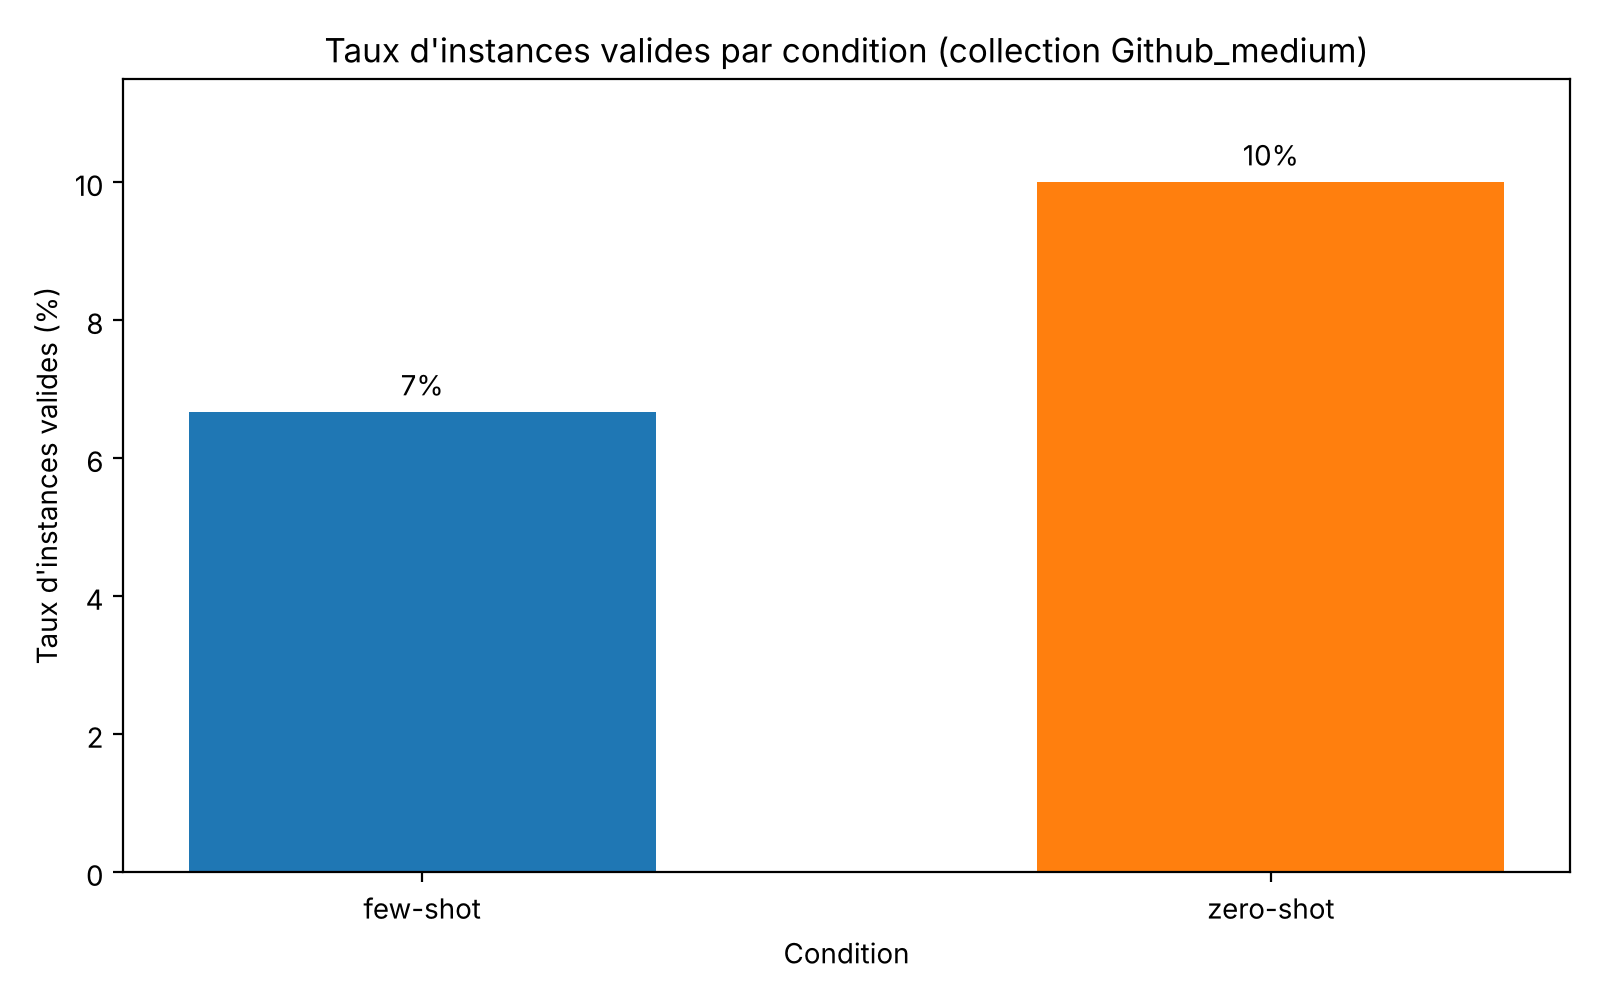
\includegraphics[width=0.75\textwidth]{plot_validite.png}
    \caption{Taux d'instances valides en zero-shot et en few-shot, sur la collection Github\_medium (30 schémas).}
    \label{fig:validite}
\end{figure}

\subsection{Les exemples utilisés en few-shot}

Les trois exemples fournis au modèle en condition few-shot ont été choisis pour rester neutres, c'est-à-dire suffisamment généraux pour ne pas orienter la réponse vers un schéma particulier du corpus testé. Ils illustrent trois formes différentes d'utilisation du \texttt{not} : sur une propriété d'un objet, sur un élément d'un tableau, et sur une chaîne de caractères.

\textbf{Premier exemple} : négation sur une propriété requise.
\begin{verbatim}
Schéma : {"type":"object","not":{"required":["deprecated"]},
          "properties":{"title":{"type":"string"}}}
Instance : {"title":"hello"}
\end{verbatim}

\textbf{Deuxième exemple} : négation sur un élément de tableau.
\begin{verbatim}
Schéma : {"type":"array","not":{"contains":{"const":"zzz"}}}
Instance : ["alpha","beta"]
\end{verbatim}

\textbf{Troisième exemple} : négation sur un motif de chaîne de caractères.
\begin{verbatim}
Schéma : {"type":"string","not":{"pattern":"^xx_"}}
Instance : "kappa"
\end{verbatim}

\subsection{Les catégories d'erreurs}

Les échecs observés relèvent de plusieurs natures différentes, ce qui a conduit à établir une classification en cinq catégories :
\begin{itemize}
    \item \textbf{overflow} : le schéma est trop volumineux pour être traité en une seule fois par le modèle ;
    \item \textbf{tronqué} : la réponse s'interrompt avant d'être complète ;
    \item \textbf{reproduction du schéma} : le modèle recopie le schéma au lieu de produire une donnée ;
    \item \textbf{mauvais contenu} : la réponse constitue un JSON valide, mais ne respecte pas une règle du schéma autre que le \texttt{not} ;
    \item \textbf{violation du \texttt{not}} : l'ensemble des contraintes est respecté, à l'exception de la valeur interdite, effectivement présente dans la réponse.
\end{itemize}

La figure~\ref{fig:categories} présente la répartition de ces catégories sur cette même collection, pour chacune des deux conditions.

\begin{figure}[H]
    \centering
    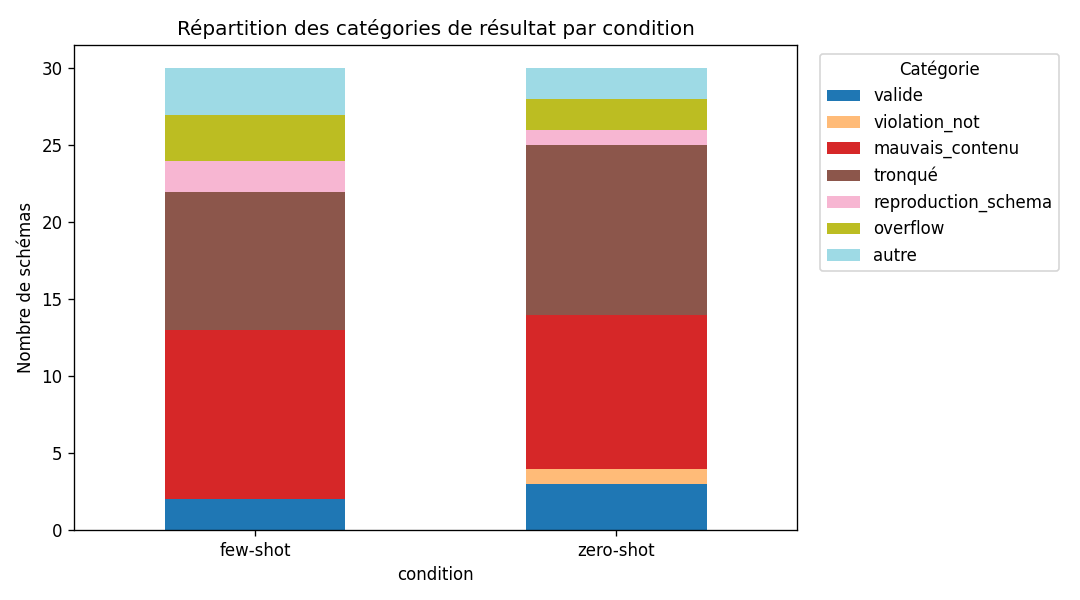
\includegraphics[width=0.8\textwidth]{plot_categories.png}
    \caption{Répartition des types de résultats en zero-shot et en few-shot, sur la collection Github\_medium (30 schémas).}
    \label{fig:categories}
\end{figure}

Il apparaît qu'une part importante des erreurs provient simplement du fait que le schéma dépasse la capacité de lecture du modèle (overflow), indépendamment de toute question liée au \texttt{not}. Ce constat a motivé une seconde expérience, plus rigoureuse, destinée à isoler l'effet propre de cette contrainte.

\section{Deuxième expérience : le \texttt{not} est-il réellement responsable des erreurs~?}

\subsection{La méthode : l'ablation}

Afin de vérifier que le \texttt{not} est bien à l'origine des erreurs observées, j'ai mené une expérience dite d'\textbf{ablation} : pour chaque schéma, une seconde version est créée, strictement identique à l'exception du \texttt{not}, qui en est retiré. Les résultats du modèle sont ensuite comparés sur les deux versions.

Lorsque le modèle réussit sur la version dépourvue de \texttt{not}, mais que sa réponse se serait révélée invalide face à la version originale (parce qu'elle contient précisément la valeur interdite), le schéma est considéré comme \textbf{bloqué par le \texttt{not}}.

Le taux de réussite passe de 10/202 avec le \texttt{not} à 18/202 sans celui-ci, soit près du double (figure~\ref{fig:ablation-global}).

\begin{figure}[H]
    \centering
    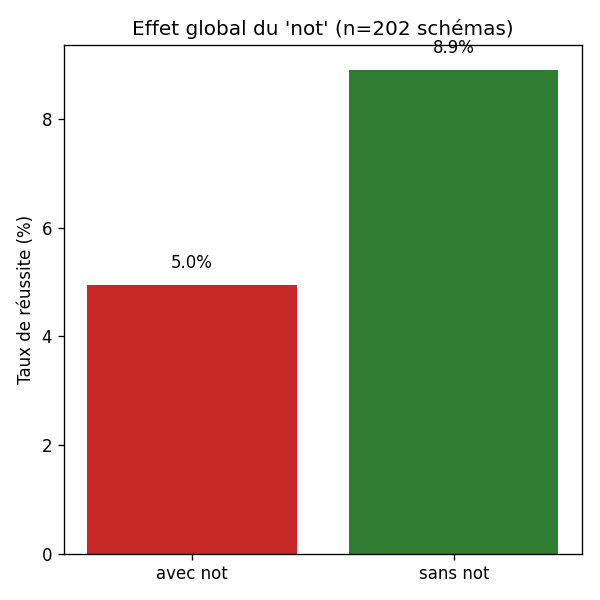
\includegraphics[width=0.36\textwidth]{plot_ablation_global.png}
    \caption{Taux de réussite avec et sans \texttt{not}, sur l'ensemble des 202 schémas.}
    \label{fig:ablation-global}
\end{figure}

La figure~\ref{fig:ablation-collections} détaille ce résultat pour chacune des collections du corpus.

\begin{figure}[H]
    \centering
    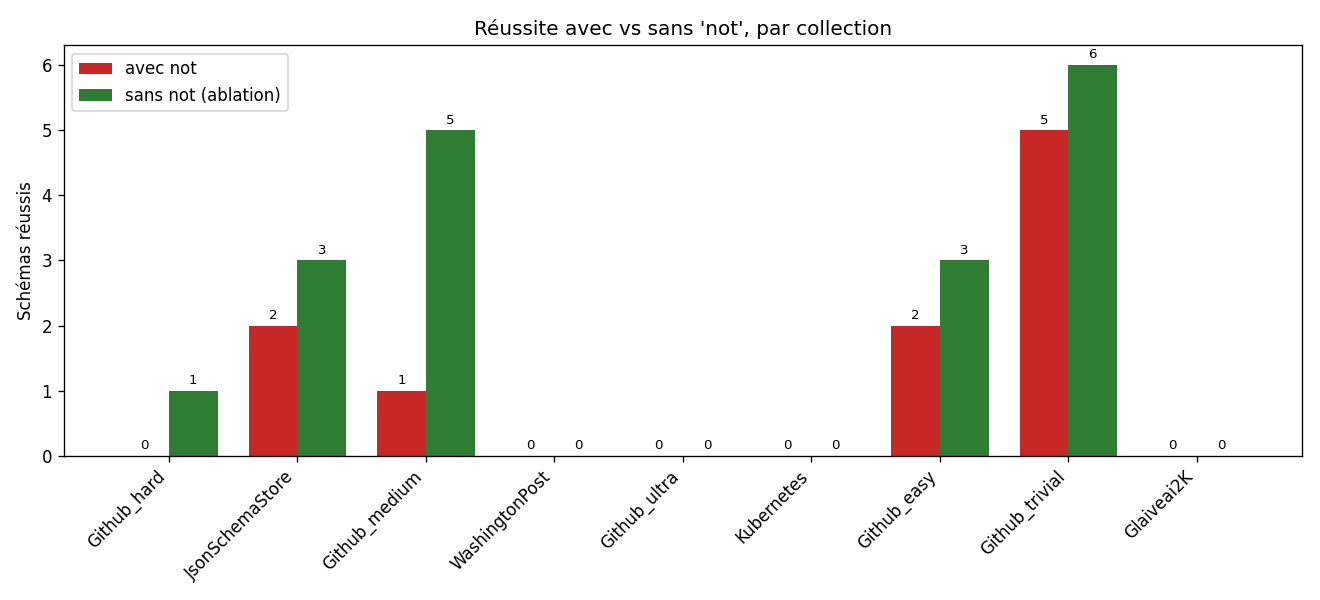
\includegraphics[width=0.72\textwidth]{plot_ablation_collections.png}
    \caption{Nombre de schémas réussis avec et sans \texttt{not}, par collection.}
    \label{fig:ablation-collections}
\end{figure}

Sept schémas ont par ailleurs été identifiés comme bloqués exclusivement par cette contrainte. Ils se répartissent entre trois collections (figure~\ref{fig:bloques}).

\begin{figure}[H]
    \centering
    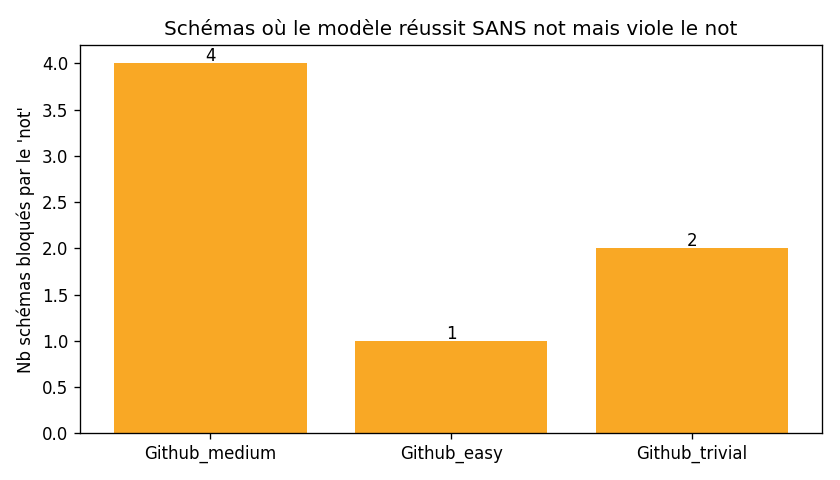
\includegraphics[width=0.6\textwidth]{plot_bloques_par_not.png}
    \caption{Nombre de schémas bloqués précisément par le \texttt{not}, par collection.}
    \label{fig:bloques}
\end{figure}

\subsection{Le few-shot améliore-t-il réellement la compréhension du \texttt{not}~?}

Une comparaison entre le zero-shot et le few-shot a également été menée sur l'ensemble ainsi constitué.

Le passage au few-shot débloque quinze schémas, mais en fait échouer quatre autres qui réussissaient auparavant, soit un gain net de onze schémas (figure~\ref{fig:fewshot}).

\begin{figure}[H]
    \centering
    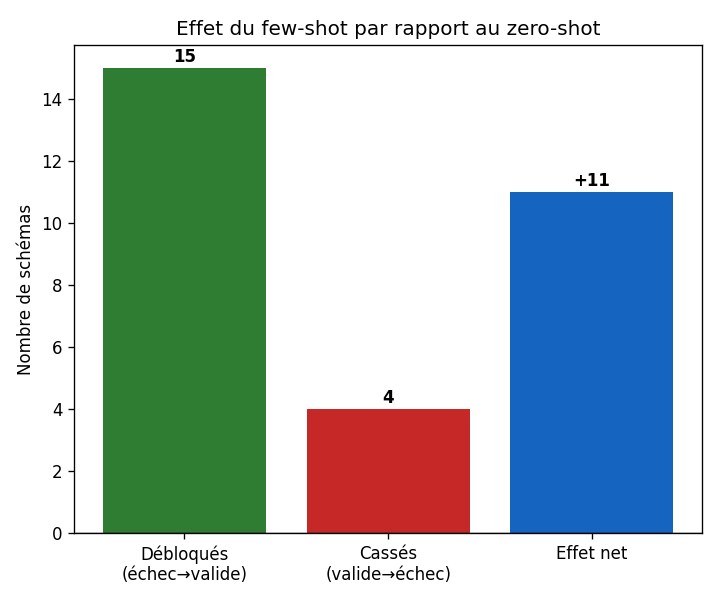
\includegraphics[width=0.6\textwidth]{plot_effet_fewshot.png}
    \caption{Effet du few-shot par rapport au zero-shot : schémas débloqués et schémas cassés.}
    \label{fig:fewshot}
\end{figure}

Toutefois, parmi les quinze schémas débloqués, seuls deux appartenaient aux sept schémas identifiés comme véritablement bloqués par le \texttt{not}. Ce résultat suggère que le few-shot améliore essentiellement la mise en forme générale du JSON produit, sans pour autant renforcer significativement la compréhension de la négation.

\subsection{Un test de reconnaissance directe}

Afin d'isoler plus nettement encore la capacité du modèle à traiter la négation, un dernier test a été mené : plutôt que de demander une génération, on soumet directement au modèle une valeur donnée et on lui demande de juger si elle est valide ou non (``valid'' ou ``invalid''), pour dix cas impliquant un \texttt{not}.

Sur les dix valeurs effectivement interdites par la contrainte, le modèle n'en a détecté \textbf{aucune}, répondant systématiquement ``valid''. Ce résultat, obtenu dans les conditions les plus simples possibles, constitue l'indice le plus net d'une difficulté réelle et spécifique du modèle à raisonner sur la négation logique.

\section{Une découverte inattendue : des schémas insatisfiables}

L'étude d'une famille de sept schémas (nommés \texttt{calculate\_area}) a révélé que le modèle échouait systématiquement à les résoudre, quelle que soit la méthode employée. Une vérification exhaustive, consistant à tester toutes les combinaisons possibles de valeurs, a permis d'en établir la cause.

Cinq de ces sept schémas se sont avérés \textbf{logiquement insatisfiables} : le schéma exige simultanément une propriété et son absence, de sorte qu'aucune donnée, aussi correcte soit-elle, ne pourrait jamais le satisfaire. Il ne s'agit donc pas d'une défaillance du modèle, mais d'un défaut de conception du schéma lui-même. Les deux schémas restants se sont en revanche révélés satisfiables, une solution valide ayant été trouvée après vérification.

\section{Construction d'une base de référence}

À la suite de ces expériences, j'ai constitué une base de données de 202 paires (schéma, donnée valide), destinée à préparer la suite du projet présentée à la section suivante. Chaque donnée a été systématiquement vérifiée à l'aide du programme de validation, tant pour s'assurer de sa conformité au schéma que pour garantir qu'elle mobilise effectivement la contrainte \texttt{not} (plutôt qu'une donnée minimale qui l'évite sans l'exercer réellement).

Pour les schémas de taille raisonnable, les données ont été rédigées manuellement. Pour les schémas les plus volumineux, dont certains dépassent 900 000 caractères, un programme a été développé pour construire automatiquement une donnée à partir des règles du schéma, puis la corriger de façon itérative jusqu'à obtenir une version valide.

Au terme de ce travail, 96\,\% des 202 données présentent un contenu réaliste et soigné, et les cinq schémas insatisfiables sont explicitement signalés comme tels dans la base.

\section{Troisième expérience : assister le modèle par des exemples pertinents (RAG)}

\subsection{Le principe}

La dernière partie de ce travail a consisté à tester une méthode appelée \textbf{RAG} (retrieval-augmented generation, soit génération augmentée par récupération). Son principe : plutôt que de fournir systématiquement les mêmes exemples au modèle, on lui propose, pour chaque nouveau schéma, les exemples les plus proches identifiés au sein de la base de 202 schémas constituée précédemment.

\subsection{Le fonctionnement du dispositif}

\begin{itemize}
    \item chaque schéma de la base est transformé en une représentation numérique (un \textbf{embedding}), permettant de comparer les schémas entre eux ;
    \item pour un nouveau schéma, les exemples les plus proches sont recherchés au sein de la base (le \textbf{retriever}) ;
    \item un texte (le \textbf{prompt}) est construit à partir de ces exemples et du schéma cible ;
    \item le modèle génère une réponse à partir de ce texte ;
    \item la validité de cette réponse est vérifiée.
\end{itemize}

Deux méthodes de calcul de similarité ont été comparées :
\begin{itemize}
    \item \textbf{MiniLM}, un modèle généraliste, sensible au sens des mots employés ;
    \item \textbf{CodeBERT}, entraîné sur du code source, davantage sensible à la structure du schéma.
\end{itemize}

\subsection{Les résultats obtenus}

Plusieurs configurations ont été testées sur un échantillon de vingt schémas (tableau ci-dessous et figure~\ref{fig:rag}) :

\begin{table}[H]
\centering
\begin{tabular}{lr}
\toprule
Configuration & Résultat \\
\midrule
Sans RAG (zero-shot) & 1/20 (5\,\%) \\
RAG avec 3 exemples, MiniLM & 6/20 (30\,\%) \\
RAG avec 1 exemple, MiniLM & 11/20 (55\,\%) \\
RAG avec 1 exemple, CodeBERT & 11/20 (55\,\%) \\
Meilleure combinaison obtenue & \textbf{12/20 (60\,\%)} \\
\bottomrule
\end{tabular}
\end{table}

\begin{figure}[H]
    \centering
    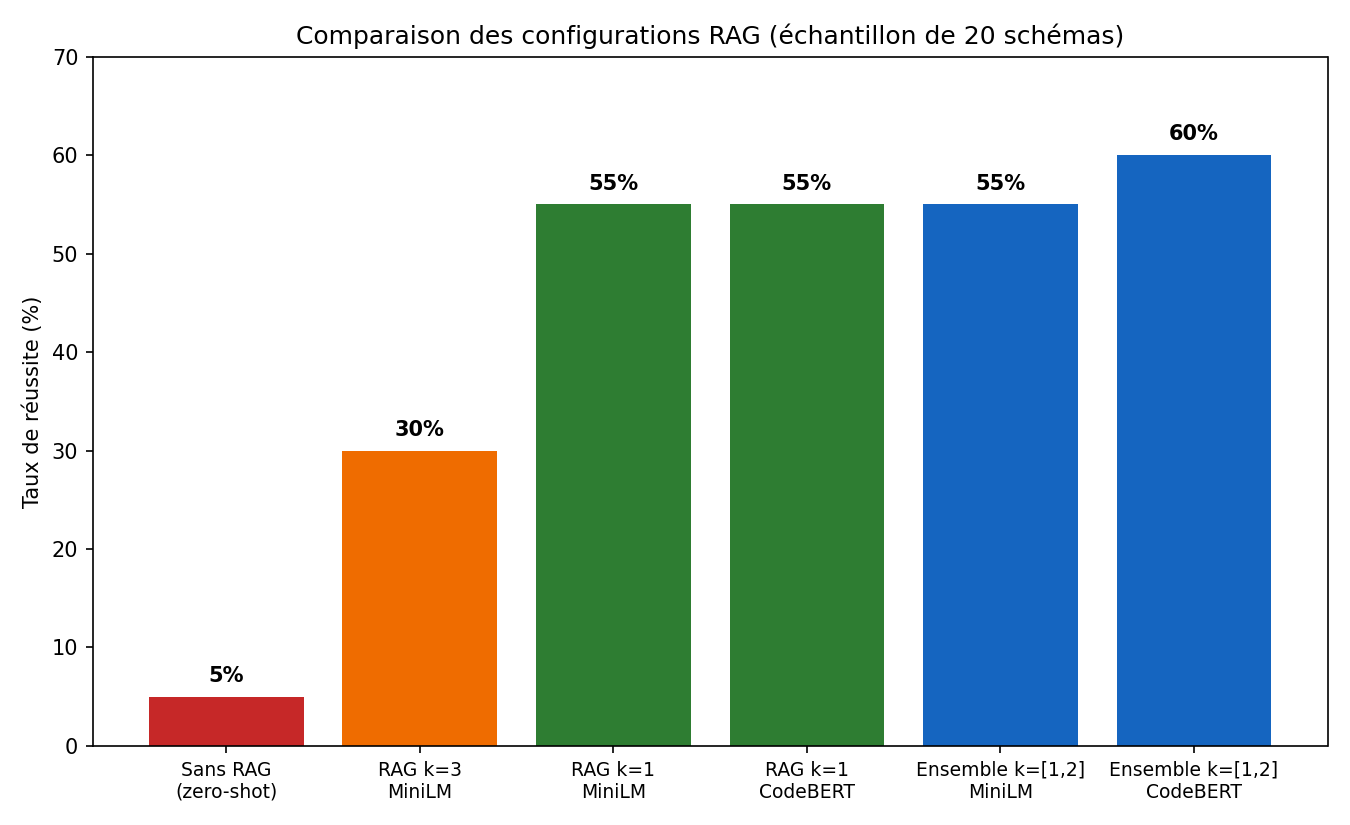
\includegraphics[width=0.85\textwidth]{plot_rag_comparaison.png}
    \caption{Comparaison des différentes configurations RAG testées.}
    \label{fig:rag}
\end{figure}

Plusieurs enseignements se dégagent de ces expériences :
\begin{itemize}
    \item le RAG améliore considérablement les résultats par rapport à l'absence de tout exemple (facteur dix environ) ;
    \item fournir un unique exemple s'avère préférable à en fournir deux ou trois. Ce résultat, à première vue contre-intuitif, s'explique par la fenêtre de contexte limitée de Phi-2 (2048 unités de texte au maximum) : plus le nombre d'exemples augmente, moins il reste de place pour que le modèle achève sa réponse, d'où une proportion croissante de réponses tronquées ;
    \item l'embedding orienté structure (CodeBERT) surpasse légèrement l'embedding généraliste (MiniLM) ;
    \item modifier la formulation des instructions données au modèle n'améliore pas les résultats, et peut même les dégrader lorsque le texte devient trop long ;
    \item en recensant précisément l'ensemble des erreurs observées, seules 35\,\% environ relèvent véritablement d'une violation du \texttt{not}. Les autres proviennent de causes distinctes (type de donnée incorrect, valeur erronée, etc.). Le \texttt{not} demeure une difficulté réelle, mais ne constitue pas, en pratique, la cause principale des échecs.
\end{itemize}

\section{Conclusion}

Ce travail met en évidence une difficulté réelle du modèle Phi-2 à traiter les contraintes de négation exprimées par le mot-clé \texttt{not}. Cette conclusion s'appuie sur plusieurs expériences convergentes : l'étude d'ablation, la comparaison entre zero-shot et few-shot, et surtout le test de reconnaissance directe, au cours duquel le modèle n'a détecté aucune des dix violations proposées.

Ce travail a également permis d'établir qu'un jeu de données, même issu de sources réelles, peut comporter des schémas logiquement contradictoires — un élément qu'il convient de vérifier avant d'évaluer les performances d'un modèle sur un tel corpus.

Enfin, la méthode RAG améliore sensiblement les résultats globaux, sans toutefois corriger spécifiquement la difficulté liée au \texttt{not} : le nombre d'erreurs de cette nature demeure comparable quelle que soit la configuration testée.

\subsection*{Perspectives}
\addcontentsline{toc}{subsection}{Perspectives}

Il serait pertinent, dans la continuité de ce travail, de reproduire ces expériences avec un modèle de plus grande taille, afin de déterminer si la difficulté observée sur le \texttt{not} tient à la taille du modèle employé, ou si elle relève d'un phénomène plus général.

\section*{Code et données}
\addcontentsline{toc}{section}{Code et données}

L'ensemble du code et des données de ce projet est disponible sur GitHub~:
\begin{center}
\url{https://github.com/zeinmil/witness-generation-bench}
\end{center}

\end{document}